\documentclass[12pt]{article}
\usepackage[english]{babel}
\usepackage[utf8]{inputenc} 
\usepackage[T1]{fontenc}
\usepackage{graphicx}
\usepackage{amsmath}
\usepackage{wrapfig}
\usepackage{enumerate}
\usepackage[top=1in, bottom=1.25in, left=1.1in, right=1.1in]{geometry}
\usepackage[dvipsnames]{xcolor}
\usepackage{subcaption}

\begin{document}

\begin{titlepage}

\newcommand{\HRule}{\rule{\linewidth}{0.5mm}} 

\center 

\textsc{\LARGE Universidad de Sonora}\\[1.5cm]
\textsc{\Large Licenciatura en Física}\\[0.5cm]
\textsc{\large Física Computacional I}\\[0.5cm]

\HRule \\[0.4cm]
{\huge \bfseries Actividad 8 - Oscilador de Van der Pol}\\[0.4cm] 
\HRule \\[1.5cm]

\begin{minipage}{0.4\textwidth}
\begin{flushleft} \large
\emph{Alumno:}\\
José Gabriel Navarro I.
\end{flushleft}
\end{minipage}
~
\begin{minipage}{0.4\textwidth}
\begin{flushright} \large
\emph{Profesor:} \\
Carlos Lizarraga Celaya
\end{flushright}
\end{minipage}\\[2cm]

09 de Abril de 2018


\includegraphics[width=0.4\textwidth]{logo.png}\\
 
\vfill

\end{titlepage}

\section{Introducción - Antecedentes}
En el presente reporte se presenta la Actividad 8 para la clase de Física Computacional I, en donde se analiza el Oscilador de Van der Pol, un oscilador con amortiguamiento no lineal, un oscilador similar a los realizados en las dos practicas anteriores. \\

Balthasar Van der Pol fue un físico neerlandés que estudió física en Utrecht en Inglaterra e ingreso en los laboratorios de Philips en 1921. Sus campos de investigación fueron la propagación de ondas, teoría de circuitos y física matemática, y su descubrimiento del oscilador que lleva a su nombre lo llevo a recibir la medalla de honor del "Institute of Radio Engineers". \\

La ecuación de Van der Pol es uno de los primeros descubrimientos de la Teoría del caos, y esta a su vez tiene una larga historia en la física y biología como mas adelante se menciona en la síntesis del artículo de Wikipedia. Además de esto, se presenta también las graficas de varios ejemplos de este oscilador y una discusión acerca de estos resultados. Por ultimo, se presentan las conclusiones al tema y el apéndice respectivo a la actividad.

\section{Modelo de Van der Pol}
El oscilador de Van der Pol es un oscilador con amortiguamiento no lineal, y obedece a la ecuación de segundo orden:

\centerline{$ \ddot x -\mu (1-x^2) \dot x +x = 0$}
$    $

En donde x es la posición, t es la función del tiempo, y $\nu$ es el amortiguamiento.

\subsection{Historia}
El oscilador de Van der Pol, como se menciono anteriormente, fue descrito por el ingeniero y físico Balthasar Van der Pol. Encontró oscilaciones estables, que nombró oscilaciones de relajación (conocidos actualmente como ciclos límite), en circuitos que usaban válvulas de vacío. Cuando se hacían funcionar a estos circuitos cerca de su ciclo límite, la señal entra en fase con la corriente, y con ayuda de uno de los colegas de Van der Pol, Van de Mark, encontraron que para ciertas frecuencias aparecía un ruido irregular siempre cerca de las frecuencias de acoplamiento. \\

Esta ecuación ha sido utilizada ya en varias áreas de la ciencia, como lo fue en Biología, donde Fitzhugh  y Nagumo crearon un modelo para describir el potencial de acción de las neuronas. Además de que este descubrimiento del ruido irregular fue uno de los primeros descubrimientos de la teoría del caos. 

\subsection{Forma Bidimensional}
Utilizando el teorema de Liénard, podemos encontrar que el sistema tiene un ciclo limite, en donde si se aplica la transformación correspondiente, podemos transformar la ecuación de segundo orden que describe este fenómeno en un sistema de ecuaciones diferenciales: \\ 

\centerline{$ \dot x = \mu(x - \frac{1}{3}x^3-y)$}
\centerline{$ \dot y = \frac{1}{\mu}x$}
$    $

O haciendo $ y= \dot x$:

\centerline{$ \dot x = y$}
\centerline{$ \dot y = \mu (1-x^2)y - x$}
$    $

\subsection{Oscilador sin forzamiento}
Existen varias características interesantes de este oscilador para estas circunstancias, una de ellas es que cuando $\mu = 0$ no hay función de amortiguamiento, por lo cual obtenemos un oscilador simple en donde si existe la conservación de la energía. \\

Cuando el valor de $\mu > 0$ el sistema entra a un ciclo limite, en donde cerca del origen el sistema esta inestable y lejos de el, esta amortiguado. \\

\subsection{Hamiltoniano para el oscilador de Van der Pol}
Se puede escribir también un Hamiltoniano independiente del tiempo para este oscilador, aumentándolo a un sistema autónomo dinámico usando ecuaciones diferenciales de segundo orden: \\

\centerline{$ \ddot x - \mu (1-x^2) \dot x + x$}
\centerline{$ \ddot y + \mu (1-x^2) \dot y + y$}
$    $

En donde se puede demostrar que el Hamiltoniano para este sistema de ecuaciones es:

\centerline{$ H(x,y,p_x,p_y) = p_x p_y +xy -\mu (1-x^2)yp_y$}
$    $

\subsection{Oscilador de Van der Pol Forzado}
El oscilador forzado de Van der Pol, al igual que en practicas anteriores, para forzarlo solamente se le añade la función $Asin(wt)$, donde A es la amplitud, y $w$ es la velocidad angular. La ecuación queda entonces: \\

\centerline{$ \ddot x -\mu (1-x^2) \dot x +x - A sin(wt)= 0$}

\subsection{Circuito Eléctrico y Caos determinista}
Para realizar el circuito descrito por la ecuación de Van der Pol, se requieren elementos del circuito activo con propiedades no lineales cubicas: $ i = \phi (v) = \gamma v^3 - \alpha v$, donde i y v son la corriente y voltaje respectivamente. Utilizando en 1920, Van der Pol construyo el oscilador con un triodo. En donde la ecuación para el circuito puede reescribirse como:  \\

\centerline{$ \ddot V - \frac{1}{C}(\alpha -3 \gamma V^2) \dot V + \frac{1}{LC}V = 0$}
$   $

En los experimentos de Van der Pol, al realizar un oscilador con forzamiento, encontró que existía caos en el sistema cuando la no-linealidad del sistema era lo suficientemente fuerte. Al realizar el circuito, Van der Pol y Van der Mark conectaron el sistema a unos receptores de telefono, en donde escucharon sonidos irregulares antes de que el periodo del sistema saltara al próximo valor. Es por eso que se dice que ellos escucharon el caos determinista antes que Edward Lorenz en 1963.

\section{Exploración de las soluciones del modelo en el Espacio Fase}
A continuación se presenta como se realizaron las graficas correspondientes a la actividad y las graficas en si, para su posterior discusión. \\

Para realizar todas las graficas se siguió el mismo principio que en las practicas pasadas, se definió un vector que almacena el sistema de ecuaciones diferenciales, se crearon varios tiempos dentro de un intervalo dado, se definieron las condiciones iniciales y por ultimo se resolvía el sistema de ecuaciones con la función de odeint. Los resultados se guardaban en un archivo y de aquí se leían para poder graficarlos:

\begin{figure}[h!]
    \centering
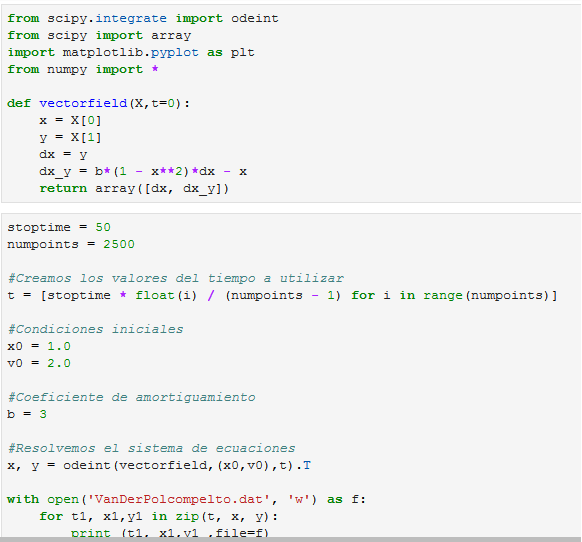
\includegraphics[width=3in]{Cod1.png}
\end{figure}

\pagebreak

Para la primera gráfica se crearon 4 archivos, ya que se presentan 4 osciladores con distintas condiciones iniciales. Para poder graficarlas, se realizo lo que ya se había hecho en practicas anteriores, solamente graficando la posición contra la velocidad. Lo nuevo de esta es que, aparece un campo vectorial, en donde en cada punto indicado aparece un vector que esta dirigido por la derivada. Para realizar esto se utilizo la función de matplot "quiver" que permite graficar estos vectores. Sin embargo, esta función solamente la genera, primeramente se tuvo que crear una cuadricula en donde se almacena los valores para la posicion y tiempo con el valor de su derivada respectiva: 

\begin{figure}[h!]
    \centering
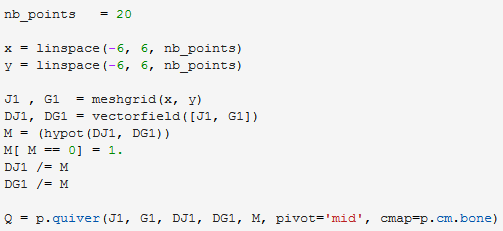
\includegraphics[width=3in]{Cod2.png}
\end{figure}

La grafica obtenida fue:

\begin{figure}[h!]
    \centering
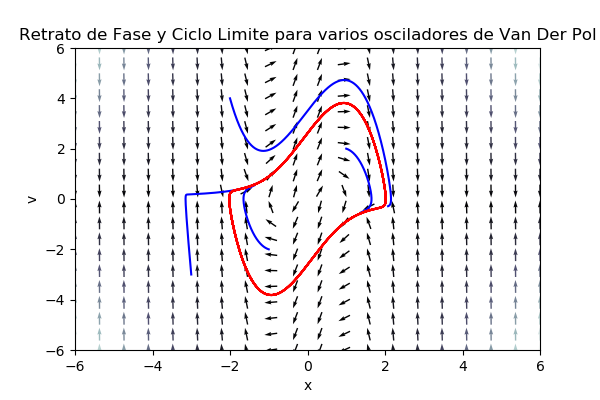
\includegraphics[width=5in]{Im1.png}
\end{figure}

Para la segunda gráfica solamente se crearon varios archivos para las distintos coeficientes de amortiguamiento, en donde se indica con colores el valor de cada una:

\pagebreak

\begin{figure}[h!]
    \centering
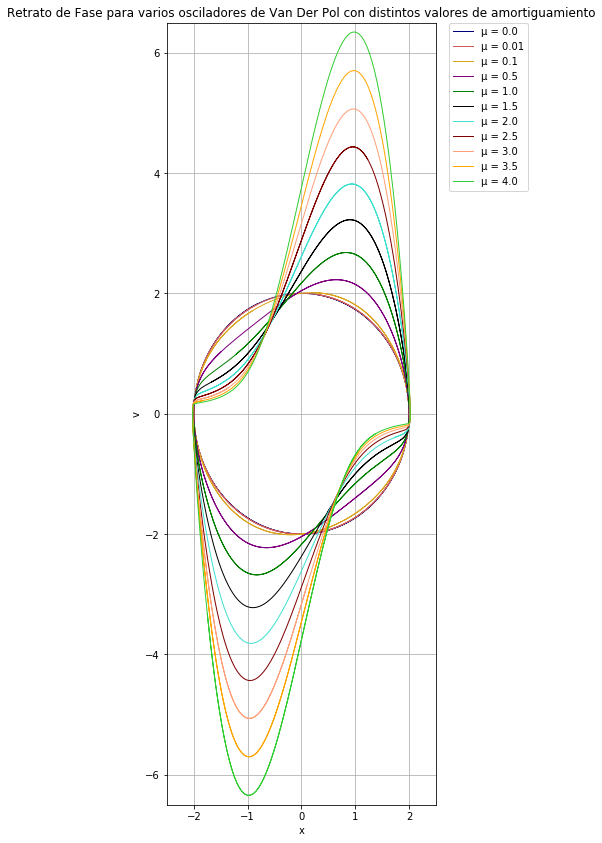
\includegraphics[width=4.5in]{Im2.png}
\end{figure}

La tercera imagen es solamente un oscilador con un valor de amortiguamiento de cinco, por lo cual solamente se genero su archivo y se creo la gráfica, lo que resulto: 

\begin{figure}[h!]
    \centering
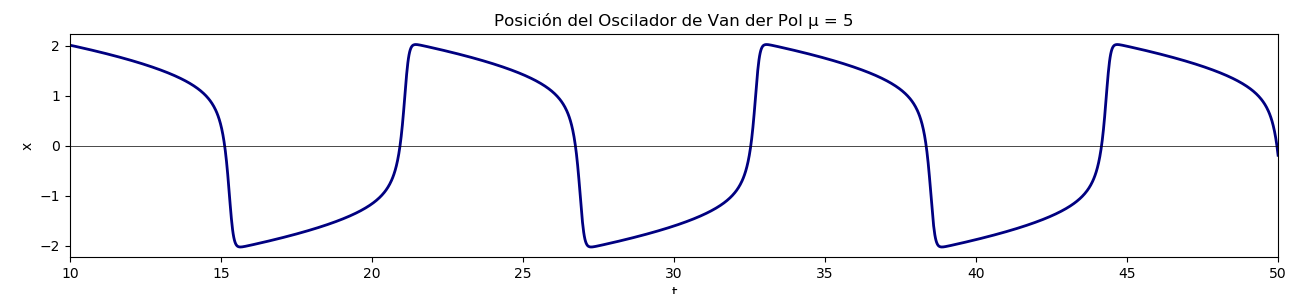
\includegraphics[width=5in]{Im3.png}
\end{figure}

\pagebreak

Por último, la ultima gráfica que se presenta en al articulo es la de un oscilador forzado con valores de $\mu$ = 8.53, A = 1.2 y $w = 2\pi/ 10$. Al vector que almacena la ecuación solamente se le agrego el valor de forzamiento anteriormente indicado, y se grafico la posición contra el tiempo:

\begin{figure}[h!]
    \centering
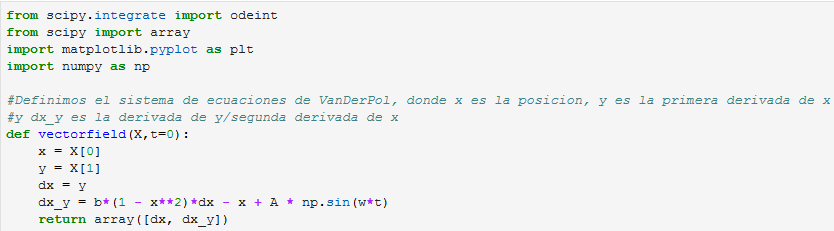
\includegraphics[width=5in]{Cod3.png}
\end{figure}

\begin{figure}[h!]
    \centering
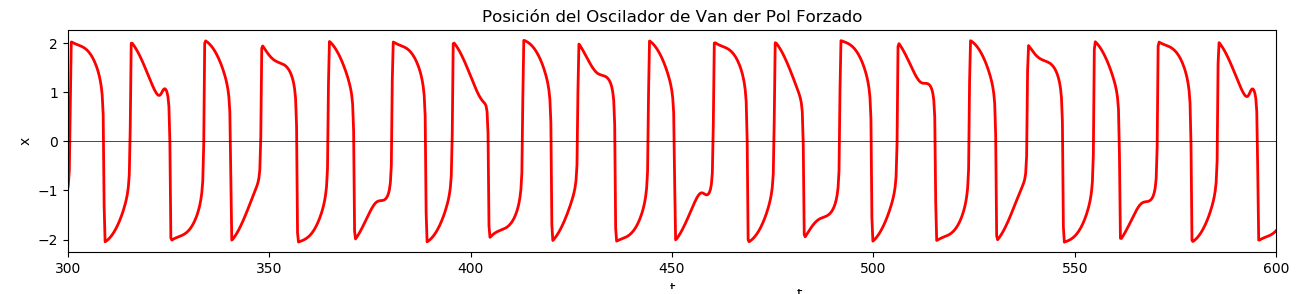
\includegraphics[width=6in]{Im4.png}
\end{figure}

\section{Resultados y discusión}
Al realizar las graficas correspondientes al articulo podemos notar distintas cosas dependiendo de cada una de ellas. Primeramente, la gráfica del campo vectorial nos indica que a pesar de tener distintas condiciones iniciales, si el oscilador tiene el mismo factor de amortiguamiento, todos tendrán el mismo ciclo limite eventualmente, tal vez no al mismo tiempo, pero eventualmente llegaran a el. Además, podemos obervar gracias al campo vectorial, que los puntos alejados al ciclo limite solo van hacia las direcciones y+ y y-, y mientras mas se acercan al limite, estas empiezan a seguir una curva. \\

La segunda gráfica nos presenta la evolución del ciclo limite para distintos valores de amortiguamiento, en donde como podemos observar este se estira cada vez mas y mas cuando el valor del amortiguamiento también aumenta. \\

La tercera y cuarta gráfica nos muestran la posición contra el tiempo del oscilador, uno que esta forzado y otro que no. Al compararlos podemos notar como el hecho de que este forzado hace cambios muy bruscos al oscilador, mientras que el que no presenta este forzamiento se comporta de una manera mas periódica. 

\section{Conclusiones del estudio}
El estudio y comprensión de este fenómeno del oscilador de Van der Pol nos permite observar como una pequeña diferencia como lo es un coeficiente de amortiguamiento permite descubrir y examinar otro tipo de información, como fue el caso de Van der Pol. Como se menciono anteriormente en el reporte, Van der Pol, al estudiar el oscilador forzado que lleva su nombre, descubrió lo que viene siendo un resultado del caos determinista. \\

El uso de estas herramientas como Python y Jupyter, permiten examinar facilmente esta información, y no solamente eso, si no tambien encontrar nueva información a partir de nuevos tipos de graficas y solucionar problemas que antes hubieran tardado dias en realizar. 

\section{Bibliografía empleada}
\begin{itemize}
    \item Van der Pol Oscillator. (2018). Recuperado de: https://en.wikipedia.org/wiki \\ /Van\_der\_Pol\_oscillator
    \item Balthasar van der Pol. (Julio 2008). Recuperado de: http://www-groups.dcs.st-and.ac.uk/history/Biographies/Van\_der\_Pol.html
    \item Van der Pol oscillator. (Enero 2014). Recuperado de: http://www.scholarpedia.org/article\\ /Van\_der\_Pol\_oscillator
    \item Leguend Guide. (2012). Recuperado de: https://matplotlib.org/users/legend\_guide.html
\end{itemize}

\section{Apéndice}
\noindent\textbf {1. Este ejercicio pareciera similar al desarrollado en las actividades 6 y 7. ¿Qué aprendiste nuevo?} \\

Como dibujar un campo vectorial para una solución de un sistema de ecuaciones diferenciales, lo cual ya se había echo anteriormente. Además de configurar distintas imágenes para que tengan el mismo diseño y tamaño que las mostradas en el articulo a recrear. \\

\noindent\textbf {2. ¿Qué fue lo que más te llamó la atención del oscilador de Van der Pol?} \\

El ciclo limite, ya que en ejemplos anteriores  este tardaba mucho en llegar a ese limite 200-300 segundos, pero aquí lo hacia en cuestión de segundos. También la forma en la que actúa la gráfica posición-tiempo del oscilador forzado, ya que cambia muy rápido y tiene un patrón curioso. \\

\noindent\textbf {3. Has escuchado ya hablar de caos. ¿Por qué sería importante estudiar este oscilador?} \\

Van der Pol y van der Mark, descubrieron que para determinadas frecuencias aparecía un ruido irregular, siempre cerca de las frecuencias de acoplamiento. Este fue uno de los primeros descubrimientos experimentales de la Teoría del caos, es por eso que es importante analizar este tipo de movimiento para poder hablar de lo que viene siendo el caos; una base para empezar a hablar de la Teoría del Caos. \\

\noindent\textbf {4. ¿Qué mejorarías en esta actividad?} \\

En general me pareció una muy buena actividad, se basa en los conocimientos que ya teníamos y el tema del que trataba es muy interesante. No mejoraría algo en particular. \\

\noindent\textbf {5. ¿Algún comentario adicional antes de dejar de trabajar en Jupyter con Python?} \\

Este lenguaje es muy extenso y actualmente es de los mas usados, por lo cual el uso y practica de este es muy importante para nuestro desarrollo como físicos. \\

\noindent\textbf {6. Cerramos la parte de trabajo con Python ¿Qué te ha parecido?} \\

Al comenzar a utilizarlo pensé que casi no tenia uso, que lo que se hacia en Python podía hacerse en otros lenguajes, pero al continuar usándolo y mirar sus distintas herramientas puedo notar ahora que este tiene muchos mas usos que análisis de datos y graficas, sino también nos puede brindar soluciones a ecuaciones diferenciales, graficar campos vectoriales y más.

\end{document}